\chapter[Green valley galaxies]{Green valley galaxies}

This work was done in collaboration with Jinfu Dai for his senior thesis 
``Exploring the green valley.''


\section{Introduction}
%%%%%%%%%%%%%%%%%%%%%%%%%%%%%%%%%%%%%%%%%%%%%%%%%%%%%%%%%%%%%%%%%%%%%%%%%%%%%%%%
%    STATEMENT OF PROBLEM
%%%%%%%%%%%%%%%%%%%%%%%%%%%%%%%%%%%%%%%%%%%%%%%%%%%%%%%%%%%%%%%%%%%%%%%%%%%%%%%%
%\section{Chemical evolution and the green valley}

The enrichment of the interstellar medium (ISM) and circumgalactic medium (CGM) 
of a galaxy involves many complicated astrophysical processes, the interplay of 
which is not yet well understood.  A critical problem in galaxy formation is to 
understand how galaxies transition from the blue sequence to the red cloud of 
the optical color-magnitude diagram.  Star formation is thought to be quenching 
in galaxies moving through the green valley, but the relevant baryonic processes 
(gas cooling, feedback, etc.) are very complex and heavily interdependent.  
Investigating the star formation history and chemical evolution of galaxies in 
the green valley should provide clues as to the evolution of a galaxy through 
the color-magnitude diagram.


%%%%%%%%%%%%%%%%%%%%%%%%%%%%%%%%%%%%%%%%%%%%%%%%%%%%%%%%%%%%%%%%%%%%%%%%%%%%%%%%
%    BACKGROUND AND RELEVANCE TO PREVIOUS WORK
%%%%%%%%%%%%%%%%%%%%%%%%%%%%%%%%%%%%%%%%%%%%%%%%%%%%%%%%%%%%%%%%%%%%%%%%%%%%%%%%
%\section{The color-magnitude diagram: Galaxies in the green valley}

Large galaxy surveys \citep[like the Sloan Digital Sky Survey;][]{York00} 
revealed the structure of the color-magnitude diagram (CMD).  As seen in Fig. 
\ref{fig:ur_CMD}, the $u-r$ CMD is dominated by two major subgroups of galaxies: 
the red cloud and the blue sequence \citep{Strateva01, Baldry04}.  Most galaxies 
that reside in the red cloud appear to be older, elliptical galaxies that are no 
longer making stars (``red and dead'').  On the other hand, the blue sequence 
consists of mostly spiral and irregular galaxies which are actively forming stars.

% u-r CMD
\begin{figure}
    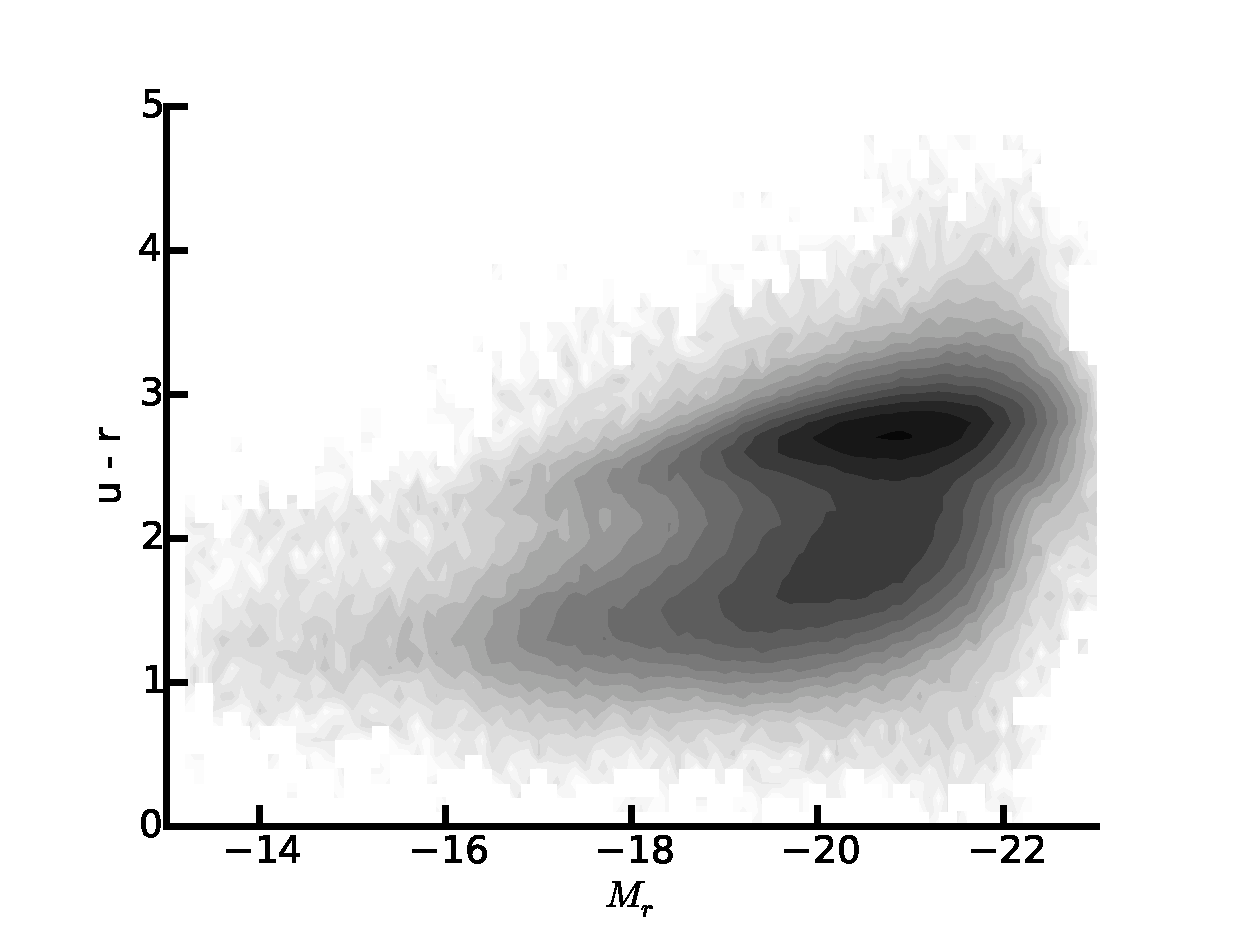
\includegraphics[width=0.49\textwidth]{Images/GV/ur_CMD_contour}
    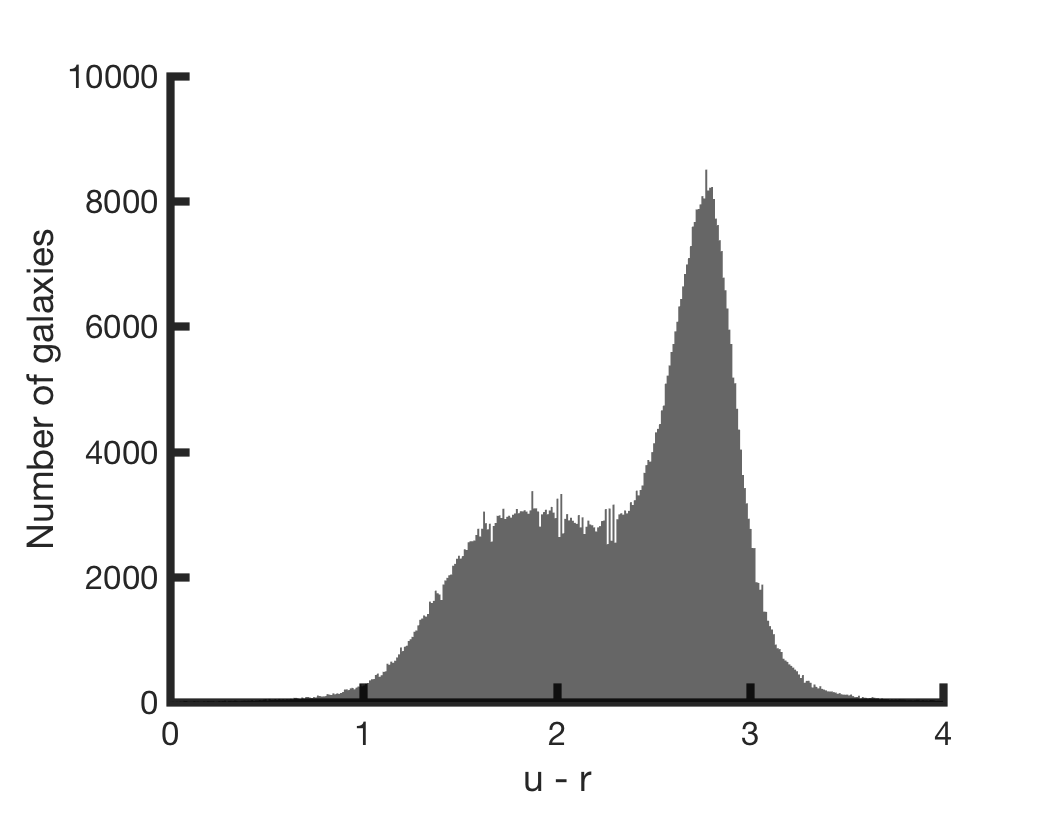
\includegraphics[width=0.49\textwidth]{Images/GV/ur_hist}
    \caption[Optical color-magnitude diagram and histogram of $u-r$ in SDSS]{The 
    optical color-magnitude diagram (left) and histogram of $u-r$ colors (right) 
    of galaxies in SDSS DR7.  There are two groups of galaxies, the populations 
    of which are well fit by the sum of two Gaussians.  They are aptly named the 
    ``red cloud'' and the ``blue sequence.''}
    \label{fig:ur_CMD}
\end{figure}

% VOGELEY THINKS THIS DESCRIPTION IS TOO SIMPLISTIC
%The current theory of galactic evolution describes a process in which a small 
%galaxy forms many stars in the beginning of its life.  As the galaxy merges with 
%others, it converts most of its hydrogen to heavier elements through 
%nucleosynthesis, and its rate of star formation slowly decreases.  The red, 
%elliptical galaxies we currently observe are hypothesized to be the remnants of 
%galaxies which have burned through the majority of their hydrogen; without fuel 
%for new stars, the galaxy's star formation rate eventually declines to a 
%negligible value.  As a result, most of the hot, massive blue stars have 
%expired, leaving behind smaller, cooler, more red stars.  These galaxies have a 
%redder color than their blue, star-forming predecessors.

% Feedback from AGN (strongly affects massive galaxies)
% Feedback from SN (dominates feedback in dwarfs)
% gas stripping interactions
% tidally-triggered star formation
There are a number of different astrophysical processes which simultaneously 
evolve a galaxy's stellar and gas content.  AGN feedback strongly affects 
massive galaxies, while dwarf galaxy feedback is dominated by supernovae.  Both 
AGN and supernovae can inject enough energy into a galaxy's ISM to prevent its 
cooling, thereby quenching star formation.  In addition to internal mechanisms, 
galaxies will often experience interactions in more dense regions.  Depending on 
the properties of the galaxies involved (mass, speed, etc.), these interactions 
can either strip gas from the galaxy (removing a primary source of fuel for 
future star formation), or they can trigger a burst of star formation.

Our current theory of galactic evolution necessitates the existence of a 
transition period in a galaxy's lifetime, when the galaxy migrates from the 
star-forming blue sequence to the red cloud on the optical CMD.  However, the 
$u-r$ CMD is very well fit by the sum of only two Gaussians \citep{Strateva01, 
Baldry04}; an intermediate population is not present in the optical CMD.  Early 
explanations developed to reconcile this apparent discrepancy between theory and 
observation included a sudden transition from the blue sequence to the red 
cloud, often associated with some star-formation quenching mechanism.

Dubbed the ``green valley,'' it is thought that star formation 
is being quenched in the galaxies moving through the green valley 
\citep{Martin07}.  So far, results of studies done with these green valley 
galaxies have been inconclusive as to why or how this is occurs.


%%%%%%%%%%%%%%%%%%%%%%%%%%%%%%%%%%%%%%%%%%%%%%%%%%%%%%%%%%%%%%%%%%%%%%%%%%%%%%%%
%%%%%%%%%%%%%%%%%%%%%%%%%%%%%%%%%%%%%%%%%%%%%%%%%%%%%%%%%%%%%%%%%%%%%%%%%%%%%%%%

\section[Data]{SDSS and GALEX data}

\subsection{Optical data --- SDSS}
%  - KIAS-VAGC (morphological classification)
% Should we use NSA for abs. mag. instead?
SDSS \citep{Abazajian09} (absolute magnitudes courtesy of the MPA-JHU 
catalog\footnote{http://www.mpa-garching.mpg.de/SDSS/DR7/})

The KIAS Value-Added Galaxy Catalog 
\citep[KIAS-VAGC]{Choi10} attempted to calculate a morphological class and type 
for all galaxies in SDSS DR7 based on the color $u-r$, color gradient 
$\Delta (g-r)$, and inverse concentration index.  

\subsection{UV data --- GALEX}
\citep{Martin05}


%%%%%%%%%%%%%%%%%%%%%%%%%%%%%%%%%%%%%%%%%%%%%%%%%%%%%%%%%%%%%%%%%%%%%%%%%%%%%%%%
%%%%%%%%%%%%%%%%%%%%%%%%%%%%%%%%%%%%%%%%%%%%%%%%%%%%%%%%%%%%%%%%%%%%%%%%%%%%%%%%


\section[Results]{Results}

Combining the results of GALEX with the optical photometry of SDSS, we construct 
a NUV$-r$ CMD.  Probing light from even younger stars in the galaxies, GALEX is 
able to increase the separation of the blue sequence and red cloud populations 
of the optical CMD, revealing a third, smaller population of galaxies 
\citep{Wyder07}.

% CMD in NUV-r, showing where green valley galaxies live
\begin{figure}
    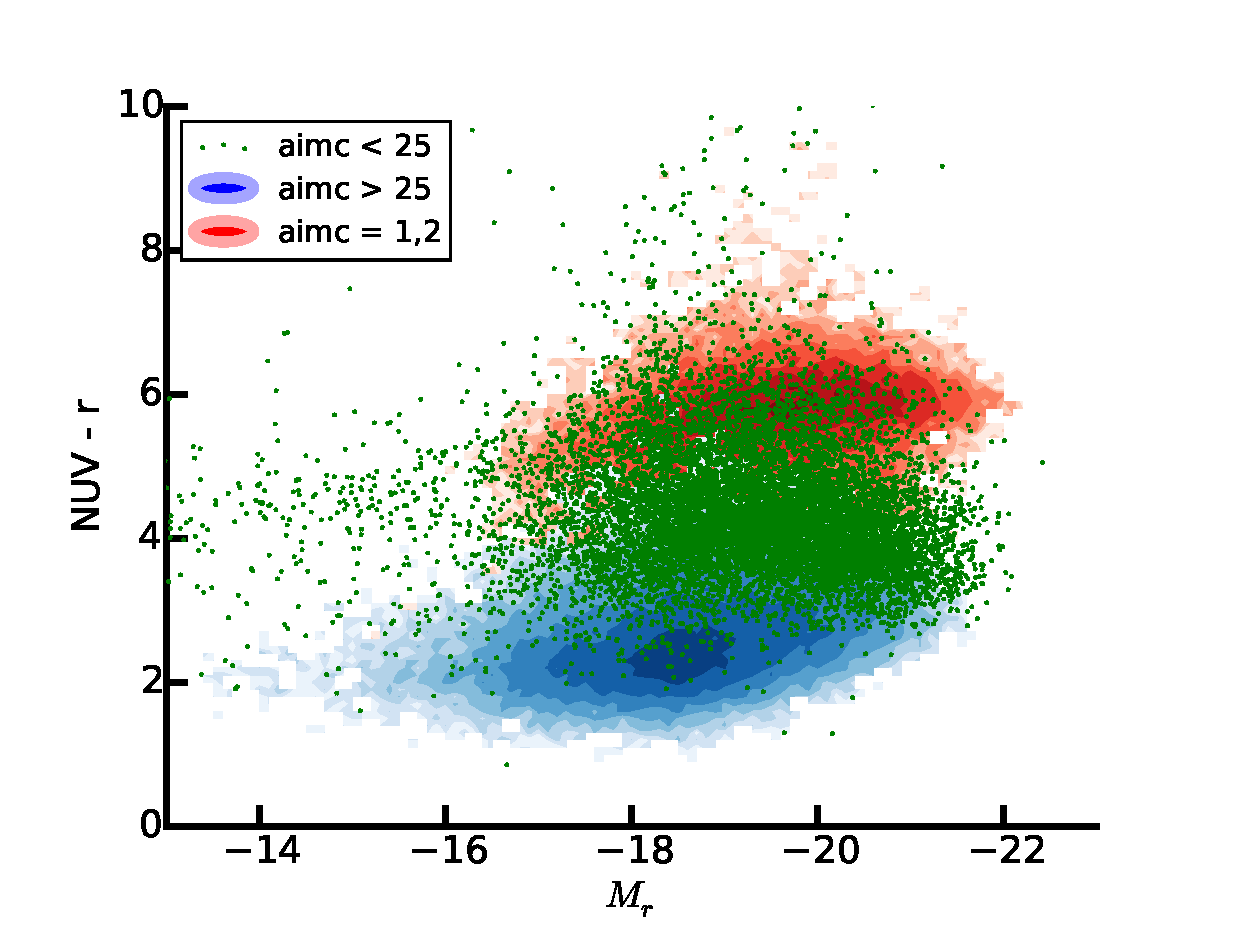
\includegraphics[width=0.65\textwidth]{Images/GV/NUVr_CMD_3pop_scatter}
    \caption[NUV-$r$ color-magnitude diagram of SDSS galaxies]{The NUV$-r$ 
    color-magnitude diagram of galaxies in SDSS DR7.  Those galaxies in the red 
    contours have morphological classifications of either normal early types 
    (aimc $=1$) or blue early types (aimc $=2$), as determined by the KIAS-VAGC.  
    The green points represent a subset of the normal late type galaxies (aimc 
    less than 25, excluding those with values of 1 or 2), and the blue contours 
    represents the remaining normal late type galaxies (aimc greater than 25).  
    It is clear that this morphological classification defines those galaxies 
    that are transitioning from the blue sequence to the red cloud.}
    \label{fig:NUVr_CMD}
\end{figure}

Preliminary analysis of mine reveals a population of galaxies that lie in the 
Green Valley on the NUV$-r$ color-magnitude diagram, identified independent of 
their location on the diagram.  I find that, rather than being 
classified based on arbitrary limits placed on the NUV$-r$ values, the galaxies 
can be easily separated into three distinct populations based on the galaxies' 
morphological types as calculated in the KIAS-VAGC; this can be seen in Fig. 
\ref{fig:NUVr_CMD}.  Defined by the $u-r$ color and the color gradient 
$\Delta (g-i)$, it is novel that an estimate of the morphological type of the 
galaxies is an adequate classification for the three populations of the NUV$-r$ 
CMD.  In addition, Fig. \ref{fig:NUVr_hist} shows a histogram of the galaxies 
which overlap in both GALEX and SDSS, separated by their morphological 
classification from the KIAS-VAGC.  It shows that the three populations are well 
fit by three Gaussians --- the new population in the middle is the transient 
galaxy population originally ``missing'' from the optical CMD.

% Histogram of NUV-r, with all, red, blue, green galaxies (aimc values)
\begin{figure}
    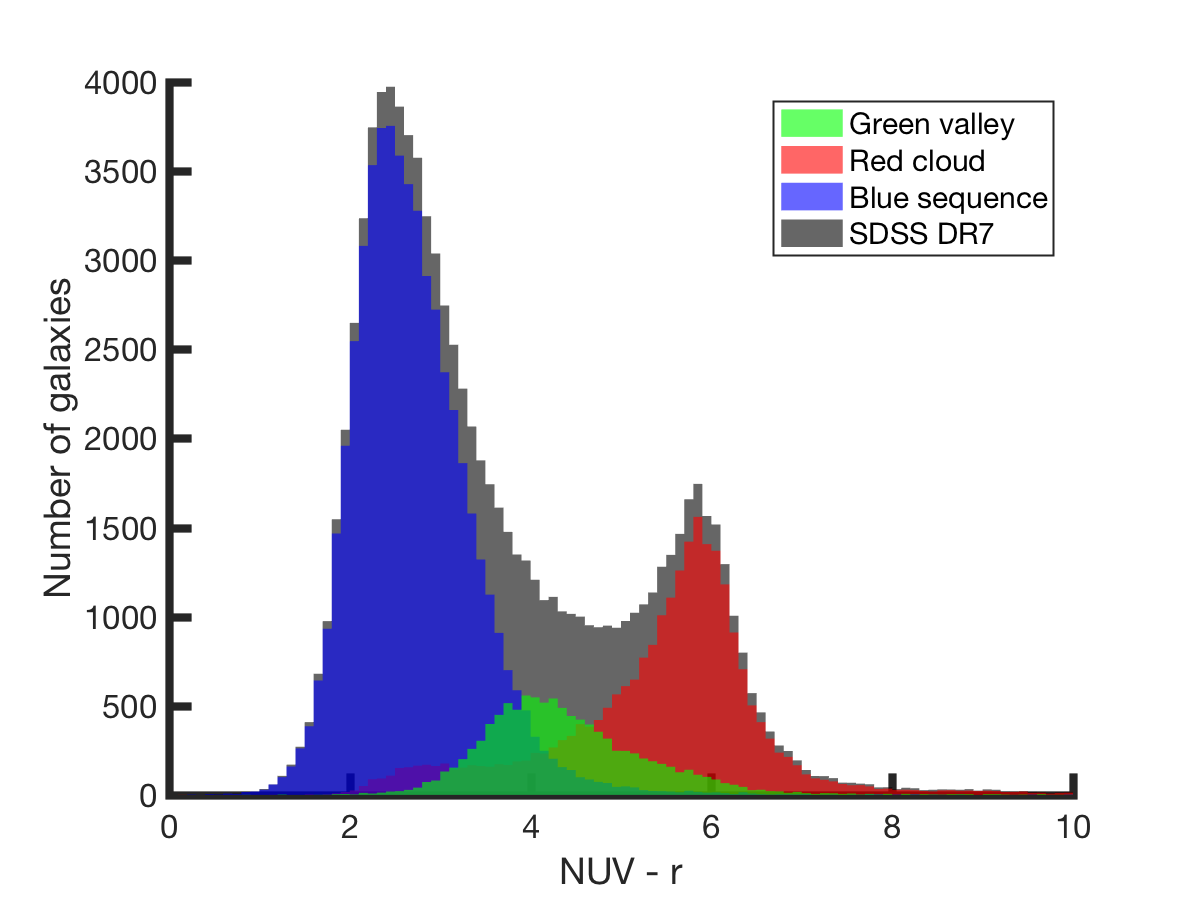
\includegraphics[width=0.65\textwidth]{Images/GV/NUVr_CMDclassifications}
    \caption[Distribution of NUV-$r$ of SDSS galaxies]{A histogram of the 
    NUV$-r$ color of those SDSS DR7 galaxies which are also detected in GALEX.  
    The red cloud, blue sequence, and green valley populations are separated by 
    the morphological types as defined by the KIAS-VAGC.  It is readily apparent 
    that the green valley galaxies exist in the space between the red cloud and 
    blue sequence.}
    \label{fig:NUVr_hist}
\end{figure}



\subsection{Large-scale environmental dependence of dwarf galaxy evolution}

Estimates of the gas-phase chemical abundances of galaxies probe their 
integrated star formation histories, which can provide insight into the 
enrichment of the ISM and CGM.  Dwarf galaxies ($M_r > -17$) have a 
slightly different evolutionary history than galaxies of large stellar masses, 
especially when looking at environmental factors.  The lower stellar masses of 
these galaxies makes them more susceptible to damage from galactic interactions 
and supernovae feedback, since they have smaller gravitational potential wells.  
My current work involves studying the large-scale environmental dependence of 
the chemical evolution of dwarf galaxies \citep{Douglass17a,Douglass17b}.  I estimate gas-phase 
metallicities (the oxygen abundance of a galaxy relative to hydrogen) with the 
Direct $T_e$ method, known for its accuracy and unbiased results.  This method 
``directly'' estimates the temperature of the electrons in an H{\sc ii} 
region from a ratio of the [O{\sc iii}] $\lambda$4363 aural line and the 
[O{\sc iii}] $\lambda \lambda$4959,5007 doublet \citep[as discussed in][this ratio 
is sensitive to the temperature of the ionized gas in an H{\sc ii} 
region]{Osterbrock89,Douglass17a}; with the temperature and density, abundance estimates can 
be made based on emission line ratios from the galaxy.  It can be very difficult 
to use, however, as it relies on a relatively strong detection of the weak [O 
{\sc iii}] $\lambda 4363$ auroral line --- the uncertainty in the measured flux 
of this emission line is the greatest source of error when using this method to 
estimate the chemical abundances.  Consequently, it is used most often on blue, 
star-forming galaxies.  A detailed description of the Direct $T_e$ method can be 
found in \cite{Douglass17a}.  We use a BPT diagram \citep{Baldwin81} to determine if a 
galaxy is star-forming or has traces of an AGN in its spectrum.  BPT diagrams 
measure the hardness of a galaxy's spectrum based on the relationship between 
ratios of some of the galaxy's emission lines.  Our star-forming classification 
is a result of the work done by \cite{Brinchmann04}.

A few of the galaxies for which I am able to estimate metallicities reside in 
the green valley.  When compared with the metallicities of galaxies in the blue 
sequence and red cloud, Fig. \ref{fig:Z_hist} shows that the star-forming green 
valley galaxies have much lower oxygen abundances than star-forming galaxies in 
the blue sequence and red cloud.  With nitrogen abundances that fall within the 
same range as the other two galaxy populations, this shift causes the N/O ratio 
to be much higher in green valley galaxies than in the others.

% Histogram of metallicity for red, blue, green galaxies
\begin{figure}
    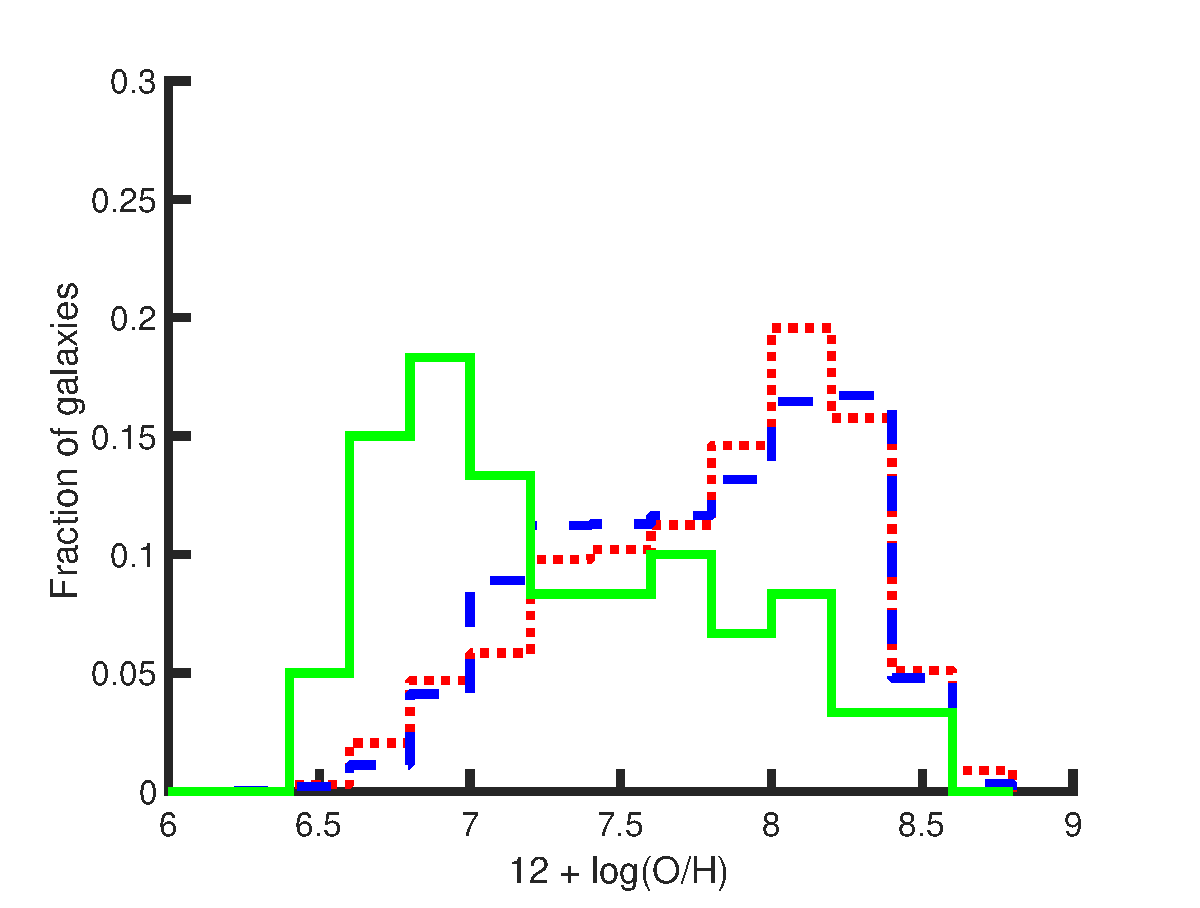
\includegraphics[width=0.49\textwidth]{Images/GV/Z12logOH_I06relations_SF_t3}
    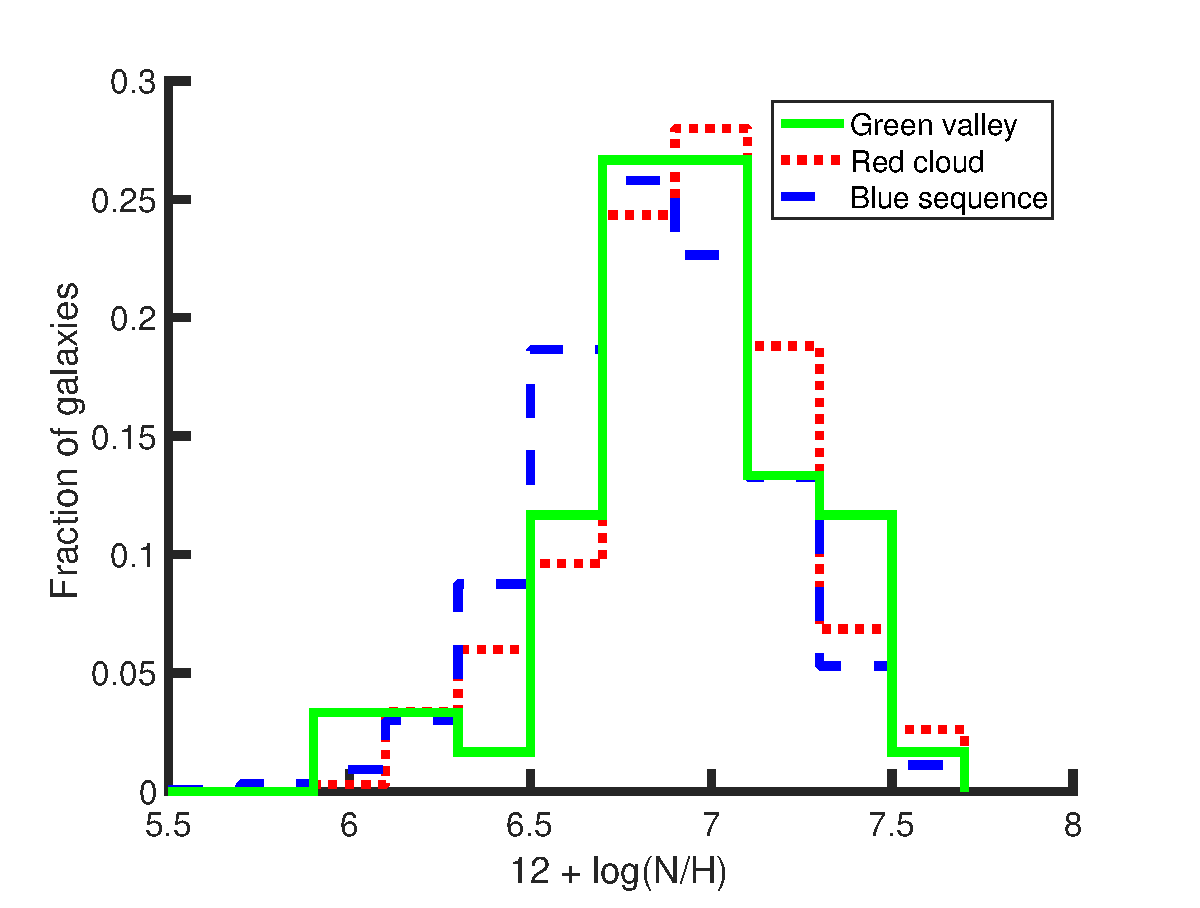
\includegraphics[width=0.49\textwidth]{Images/GV/N12logNH_I06relations_SF_t3}
    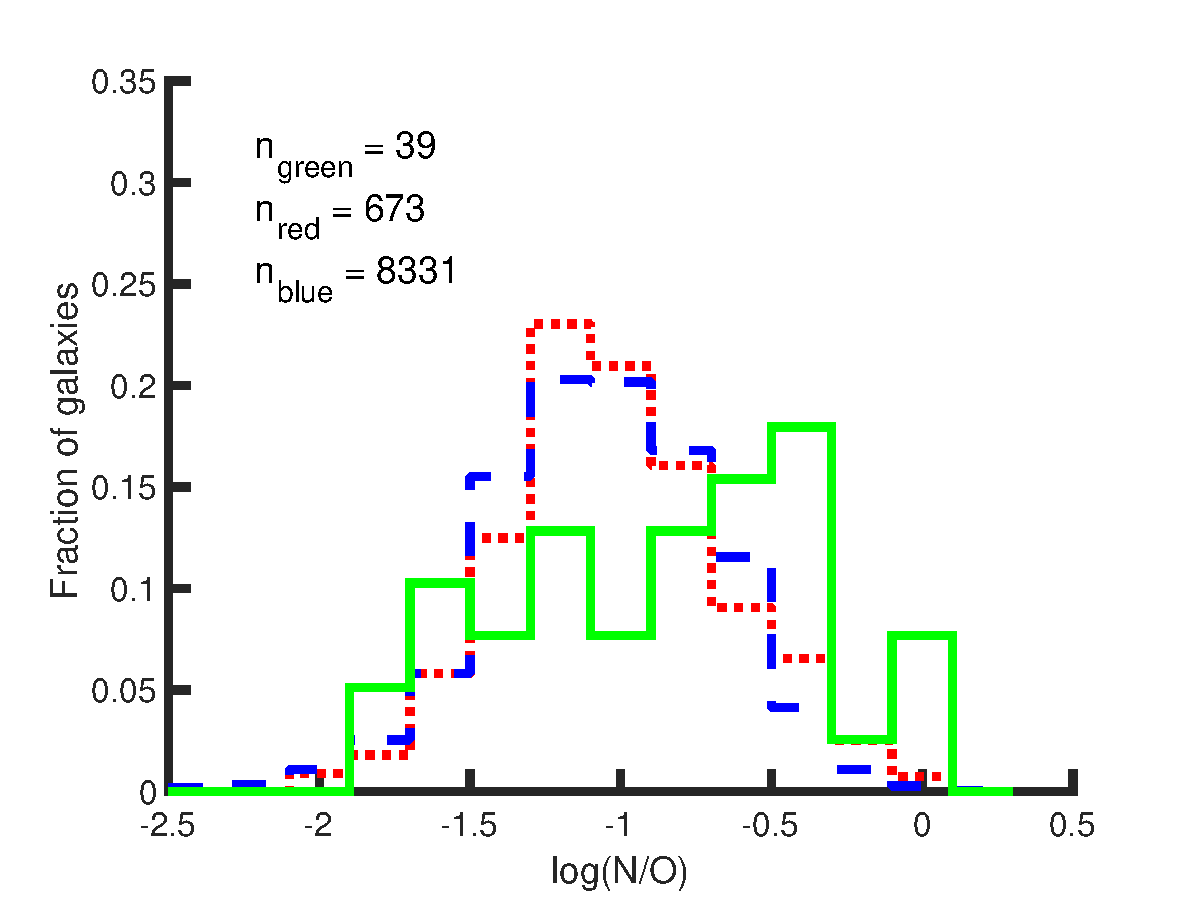
\includegraphics[width=0.49\textwidth]{Images/GV/logNO_I06relations_SF_t3}
    \caption[Distribution of gas-phase chemical abundances in cross-matched SDSS 
    DR7 -- GALEX galaxies]{Histograms of the oxygen abundance (top left), 
    nitrogen abundance (top right), and N/O ratio (bottom center) of the 
    cross-matched SDSS DR7 -- GALEX galaxies (both dwarf galaxies and brighter 
    systems), separated into their locations on the NUV$-r$ color-magnitude 
    diagram according to the morphological type listed in the KIAS-VAGC.  It is 
    readily apparent that the green valley galaxies have much lower oxygen 
    abundances than those in the blue sequence or red cloud.  This, therefore, 
    corresponds to them having the highest N/O values of the three categories.}
    \label{fig:Z_hist}
\end{figure}

When we separate the galaxies in each of the three populations by their 
large-scale environment, we discover a variation in these populations as a 
function of luminosity.  Galaxies are divided into one of two categories for 
their large-scale environment: voids or walls (more dense regions) based on the 
void catalog compiled by \cite{Pan12}.  This void catalog is constructed from 
SDSS DR7 using the VoidFinder algorithm of \cite{Hoyle02}.  As we see in Fig. 
\ref{fig:Mr_bin}, the fraction of galaxies in the green valley depends on the 
large-scale environment, even at fixed stellar mass or luminosity.  A larger 
fraction of wall dwarf galaxies are found in the green valley than for void 
dwarf galaxies.

% Fraction of red, green, blue galaxies binned by Mr in voids, walls
\begin{figure}
    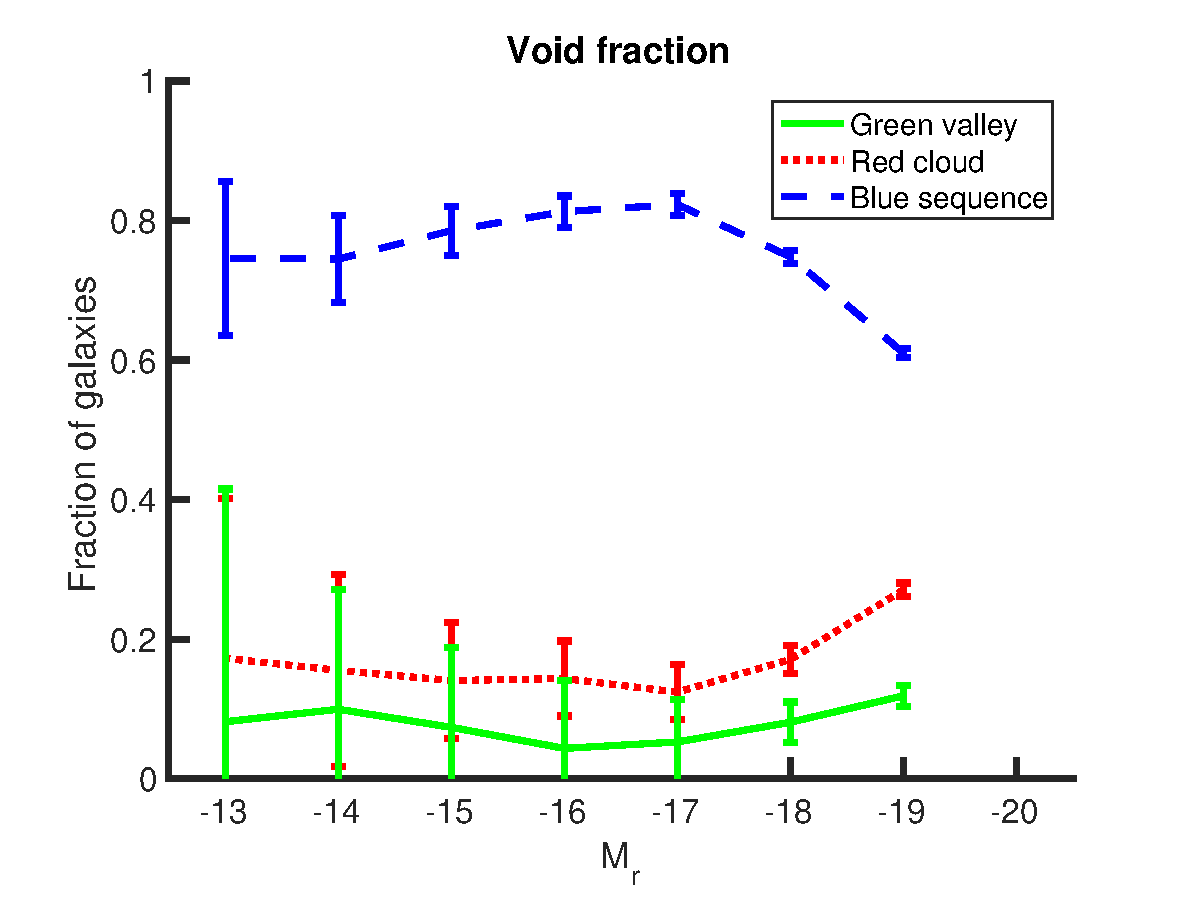
\includegraphics[width=0.49\textwidth]{Images/GV/voidFrac_CMD}
    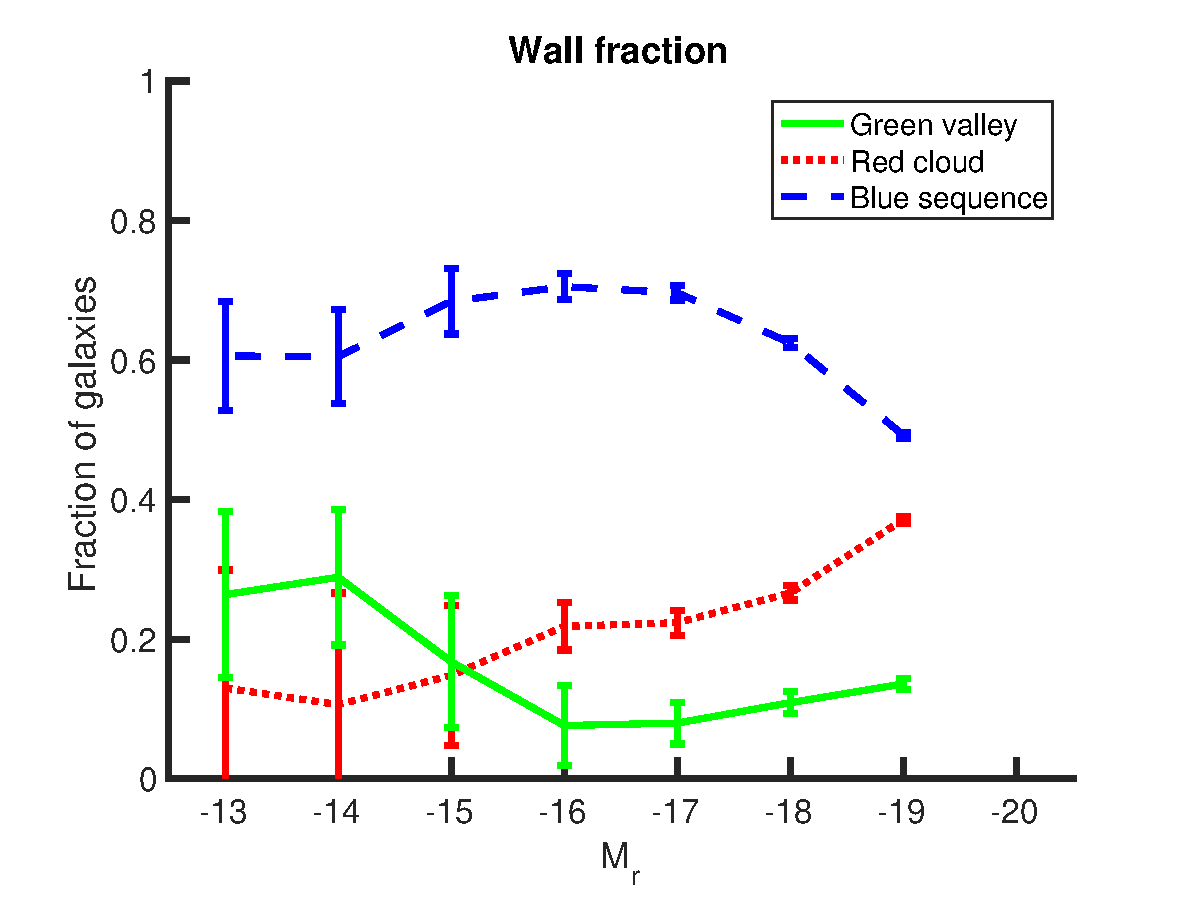
\includegraphics[width=0.49\textwidth]{Images/GV/wallFrac_CMD}
    \caption[Fraction of galaxies in CMD populations by morphological type]
    {Fraction of void (left) and wall (right) galaxies in each of the three CMD 
    populations, classified by the morphological type listed in the KIAS-VAGC.  
    There is a higher fraction of green valley dwarf galaxies ($M_r > -17$) 
    found in the more dense environments than in the voids.  This would indicate 
    that void galaxies are slightly behind wall galaxies in their evolution, 
    matching predictions based on the $\Lambda$CDM cosmology.}
    \label{fig:Mr_bin}
\end{figure}



%%%%%%%%%%%%%%%%%%%%%%%%%%%%%%%%%%%%%%%%%%%%%%%%%%%%%%%%%%%%%%%%%%%%%%%%%%%%%%%%
%%%%%%%%%%%%%%%%%%%%%%%%%%%%%%%%%%%%%%%%%%%%%%%%%%%%%%%%%%%%%%%%%%%%%%%%%%%%%%%%


\section[Discussion]{Discussion}


\subsection{Morphological classification and gas content indicators}

% classical classification of morphology v. aimc (aimc appaers to be a good indication of the transition in galaxy evolution
% Are there other markers in the gas content of these galaxies?

The morphological classification that we use to isolate the green valley 
population is relatively unique in that it is analytic; morphological 
classification attempts are often completed in a more subjective manner 
\citep[such as the GalaxyZoo,][]{Lintott11}.  In particular, the 
morphological type provided in KIAS-VAGC is a combination of the color $u-r$ and 
the color gradient $\Delta (g-i)$.  Both these quantities are independent of the 
NUV$-r$ CMD, which is part of the novelty behind why this measure separates the 
galaxies into the three evolutionary stages of the CMD so well.

%I also plan to search for other markers in the gas content of the galaxies in 
%the green valley.  
If a galaxy's star formation is quenched due to a loss of 
cold gas, then its H{\sc i} content will be lower than other galaxies of a 
similar stellar mass and large-scale environment.  If it is quenched due to a 
high gas temperature (from AGN or supernovae feedback), then the temperature of 
the gas will be higher than others of a similar size.  These factors will also 
help to determine when and why a galaxy transitions from star-forming to 
quiescent (and maybe back to star-forming).


\subsection{Testing for evidence of AGN feedback}

During my estimation of the chemical content of galaxies with $M_r > -20$, I 
note that the oxygen abundances of galaxies classified as AGN by their 
emission line ratios in the BPT diagrams exhibit extremely low oxygen abundances 
(but normal nitrogen abundance values) when compared to star-forming galaxies of 
a similar stellar mass and large-scale environment.  The same abundance 
signature is seen in the the oxygen and nitrogen abundance results seen in Fig. 
\ref{fig:Z_hist} of the green valley galaxies.  This might indicate a 
link between some dwarf green valley galaxies and a host AGN.  This 
would support other studies of the transition of galaxies from the blue sequence 
to the red cloud, which attribute the quenching of star formation to accretion 
of a central black hole.

I expect to find a large-scale environmental effect on the star formation 
quenching mechanism in addition to the AGN effects.  Giving us feedback on the 
role of the environment in a galaxy's evolution, these results will have great 
impact on the input parameters of large hydrodynamic simulations.  This project 
will serve as an example of the possible science that will be able to be done 
with the future James Webb Space Telescope.



%%%%%%%%%%%%%%%%%%%%%%%%%%%%%%%%%%%%%%%%%%%%%%%%%%%%%%%%%%%%%%%%%%%%%%%%%%%%%%%%
%%%%%%%%%%%%%%%%%%%%%%%%%%%%%%%%%%%%%%%%%%%%%%%%%%%%%%%%%%%%%%%%%%%%%%%%%%%%%%%%


\section[Conclusion]{Conclusion}